\section{One platform: \FluxCloud/\FluxEdge convergence, one provider runtime, and the datacenter tier}
\label{sec:one-platform}

The roadmap names Q4 2026 the quarter in which ``the platform becomes one product''
\srcroadmap{flux-roadmap-public.md:41}. Read literally, that is a claim about two products merging
their sign-up flows. Read structurally, it is a claim about two runtimes — one that places Docker
containers by gossip and self-selection, one that rents Kubernetes-scheduled compute by the second
— being asked to speak one protocol to the fleet they both run on. This section takes the second
reading and argues it on its own terms: today there are two products, two orchestration models, and
one network of collateralised machines underneath both. The interesting question is not whether the
two products get one web front end; it is whether a single runtime can advertise what a node can do
and let placement decide what runs where. The paper's claim is that convergence, properly stated, is
an architectural proposition about a capability-typed provider runtime, not a UI decision — and that
the concrete evidence for it is thin enough that the honest thing to do is describe exactly what
exists, what is drafted, and what has not been designed at all.

\subsection{What the two things actually are today}

\FluxOS is a per-node orchestration daemon: every Flux node runs an independent Node.js process that
exposes an HTTP/HTTPS API, gossips application state over a signed peer-to-peer mesh, and decides —
with no central scheduler — whether to pull and run a given application's Docker containers
(\shipped, \srccode{flux/\allowbreak{}ZelBack/\allowbreak{}src/\allowbreak{}services/\allowbreak{}appLifecycle/\allowbreak{}appInstaller.js}{415-746}). Placement is
opportunistic self-selection: a node scans for applications short of their required instance count,
picks among the eligible candidates largely at random, broadcasts an installing-intent message, waits
90 seconds for that message to propagate, and only proceeds if its own broadcast rank still fits the
remaining slots — earliest-broadcast-wins, with no leader election and no on-chain arbitration
(\shipped, \srccode{flux/\allowbreak{}ZelBack/\allowbreak{}src/\allowbreak{}services/\allowbreak{}appLifecycle/\allowbreak{}appSpawner.js}{254-336, 666-684}). This
runs today across a fleet measured at 6,489 nodes
(\srcmeasured{api.runonflux.io/\allowbreak{}daemon/\allowbreak{}listzelnodes}{2026-09-03}; Section~9 gives the full mechanism).

\FluxEdge, in code, is not a variant of this. It is \texttt{pouwbackend}, a Go monolith that
orchestrates rented compute through Rancher/Kubernetes: a documented OpenAPI~3.1.1 REST surface
(\texttt{GET~/gpus}, \texttt{POST~/\allowbreak{}rental/\allowbreak{}start}, \texttt{POST~/\allowbreak{}deployment/\allowbreak{}start}, and siblings),
bearer-token authentication with enumerated, per-key privileges (\texttt{start\_rental},
\texttt{stop\_rental}, \texttt{start\_deployment}, \texttt{stop\_deployment}, \texttt{get\_balance})
enforced against each request's path (\shipped,
\srccode{pouwbackend/\allowbreak{}rest\_api/\allowbreak{}v1/\allowbreak{}openapi.yaml}{2571-2581};
\srccode{pouwbackend/\allowbreak{}rest\_api/\allowbreak{}ratelimit.go}{375-390}), and GPU assignment via Kubernetes
device-plugin resources — a pod requests \texttt{nvidia.\allowbreak{}com/\allowbreak{}gpu:\allowbreak{}~N}, and the backend reconciles that
count against the rented machine's physical inventory by writing
\texttt{NVIDIA\_VISIBLE\_DEVICES} directly (\shipped,
\srccode{pouwbackend/\allowbreak{}rancher/\allowbreak{}deployment.go}{914-982}). Isolation is whole-device: there is no MIG,
vGPU or time-slicing code anywhere in the repository, and on contention the GPU resource request is
silently stripped from the pod spec rather than queued or refused — a workload can be scheduled
without the accelerator it asked for, with no error surfaced to the caller (Section~15 gives this its
own treatment).

These are two different orchestration models — gossip-and-self-select over Docker versus
API-driven Kubernetes rental — not two skins on one placement engine. That difference is exactly why
convergence is an architectural claim rather than a rebrand: unifying the interface a tenant sees does
not by itself unify how a workload gets a machine.

The two stacks are already physically coupled, though: \FluxEdge's own contractor-authored
GitOps repository packages \FluxAI's inference models (Llama~3.1, DeepSeek, FluxOne/Flux.1-dev) as
Kubernetes manifests deployed through an Argo workflow whose node-selection parameters are
documented as injected ``dynamically'' by \FluxEdge at submission time (\shipped,
\srccode{fluxai-fluxedge/\allowbreak{}custom-workflow-fluxone.yaml}{7-9,17-18}). \FluxAI's own inference capacity
runs as workloads on \FluxEdge nodes today (\shipped\ for the manifests and node-selection contract;
the exact system that submits the workflow was not independently confirmed against \FluxEdge's own
source, \srcinferred\ for that specific link). So the self-hosting relationship the roadmap gestures
at when it says the platform becomes one product is, in one narrow and already-shipped sense, real:
Flux's own AI product already depends on \FluxEdge capacity. What is not established is that a
tenant-facing workload can move between the two runtimes, or that either runtime knows the other's
resource model.

\subsection{``One provider runtime'', concretely}

The only concrete artifact for the convergence claim is a small, brand-new specification: the
\emph{Provider Runtime Contract v0}, in the \texttt{flux-spec} repository, alongside the unrelated
v9 application-specification schema described in Section~10. The repository's own README states its
status without qualification: ``Status: RFC-0 — draft for comment (2026-09-01). Not live on the
network'' (\inprogress, \srcdoc{flux-spec/README.md:3}). At the time of this survey the repository is
two days old — its entire git history is two commits, both on 2026-09-01
(\srccode{flux-spec (git log)}{706db1d, dbaf9cb, 2026-09-01}) — and the package manifest declares
\texttt{"private":\allowbreak{}~true} with no \texttt{bin}, \texttt{main} or \texttt{exports} field, meaning no
other Node.js project can currently \texttt{require} it (\inprogress, as a fact about the code today,
\srccode{flux-spec/\allowbreak{}package.json}{1-12}). Nothing in the corpus reads it: it is not the schema the
more mature \FluxOS \texttt{feat/fluxos-v9} fork actually vendors for its own application-spec
validation, which is a separate, private, commit-pinned monorepo
(\srcbranch{MorningLightMountain713/\allowbreak{}flux}{feat/fluxos-v9}{package.json:87-90}), and no repository in this survey imports
or calls into the provider-runtime schema specifically. \inprogress\ is the honest tag: it is a
complete, independently-executable artifact, not vision language, but it has no consumer.

The provider-registration schema names eleven fields, three of them nested inside
\texttt{capabilities} and two inside each entry of the optional \texttt{attestations} array
(\inprogress, \srccode{flux-spec/\allowbreak{}provider-runtime/\allowbreak{}provider-registration.schema.json}{7-80}):

\begin{center}
\begin{tabular}{ll}
\toprule
Field & Constraint \\
\midrule
\texttt{contract\allowbreak{}Version} & \texttt{const:~0}, not upwards-compatible \\
\texttt{providerId} & string, opaque to the platform, $\le$128 chars \\
\texttt{capabilities.\allowbreak{}bonded} & boolean \\
\texttt{capabilities.\allowbreak{}gpu} & boolean \\
\texttt{capabilities.\allowbreak{}staticIP} & boolean \\
\texttt{heartbeat\allowbreak{}Interval\allowbreak{}Seconds} & integer, $[10,300]$ \\
\texttt{attestations[]} & optional; absence = standard trust tier \\
\quad\texttt{.evidenceType} & open string token, not a closed enum \\
\quad\texttt{.reference} & string, $\le$512 chars \\
\texttt{payout\allowbreak{}Destination} & string, $\le$128 chars (a ZelID today) \\
\bottomrule
\end{tabular}
\end{center}

A provider that has registered is tracked by a heartbeat state machine, defined entirely in prose in
the companion contract document, with no implementation anywhere in the repository
(\inprogress, \srccode{flux-spec/\allowbreak{}provider-runtime/\allowbreak{}contract.md}{63-85}):

\begin{center}
\begin{tabular}{lll}
\toprule
State & Trigger in & Trigger out \\
\midrule
on-time & authenticated message within interval & interval expires with no heartbeat $\to$ \textsc{late} \\
\textsc{late} & recorded, no action taken & 3 consecutive expired intervals $\to$ \textsc{suspended} \\
\textsc{suspended} & no new work assigned; in-flight work runs to its booking boundary & 10 consecutive
expired intervals (total) $\to$ \textsc{lapsed} \\
\textsc{lapsed} & registration removed from scheduling & only path back is a fresh, full registration \\
\bottomrule
\end{tabular}
\end{center}

A heartbeat is defined payload-agnostically as ``any authenticated message from the provider within
the interval'' \srcdoc{flux-spec/provider-runtime/contract.md:67-69}, and ``clock authority is the
platform's'' \srcdoc{flux-spec/provider-runtime/contract.md:83} — a provider that declares too short
an interval only hurts itself. Attestation absence never blocks entry; it caps trust tier, a
permissive-by-absence rather than deny-by-default posture \srcdoc{flux-spec/provider-runtime/contract.md:39,121-123}.
The document also records a five-business-day sign-off window between the FluxCore team and the
operator submitting a contract, with the explicit fallback that an elapsed window without sign-off is
recorded as ``contract unilaterally published, sign-off pending'' rather than blocking work
\srcdoc{flux-spec/provider-runtime/contract.md:144-155} — a governance process, not a technical
guarantee, and one with no enforcement code anywhere.

\subsection{Capability flags as the architectural argument}

The claim worth making precisely is this: if one runtime advertises what a node can do — GPU
presence, machine class, network-grade, storage durability — placement stops being ``which of two
systems handles this request'' and becomes a constraint-satisfaction problem over one heterogeneous
fleet. That requires three things to exist together: a capability vocabulary a provider can declare
against, an advertisement protocol that gets the declaration (and its changes) to whoever places
work, and a placement algorithm that actually reads the vocabulary when it chooses a node. Only the
first two are drafted, and even the vocabulary is thinner than the full list above.

\textbf{Vocabulary: drafted, and narrow.} The provider-runtime contract's \texttt{capabilities} object
carries exactly three boolean flags — \texttt{bonded}, \texttt{gpu}, \texttt{staticIP} — and the v9
application schema separately carries a three-value \texttt{machineType} enum,
\texttt{standard}\,|\,\texttt{gpu}\,|\,\texttt{vps} (\inprogress,
\srccode{flux-spec/\allowbreak{}schema/\allowbreak{}v9.json}{79-82}). Nothing named ``datacenter-grade networking'' or
``persistent storage'' exists as a provider capability flag in either schema: persistent storage is
expressed today as a per-component \texttt{volumes} request on the tenant side, not as something a
provider advertises, and ``datacenter-grade'' is roadmap prose, not a schema token. A working
capability vocabulary for the fleet described in this section would need to grow considerably before
it covered what the roadmap's own language implies.

\textbf{Advertisement protocol: drafted.} Registration is the advertisement act, and the heartbeat
keeps it alive — but because a heartbeat is defined as payload-agnostic (any authenticated message
within the interval), the contract does not specify whether a provider updates its declared
capabilities by heartbeat or must re-register to change them. That is an open question the draft
leaves open, not a gap this paper is inventing.

\textbf{Placement algorithm: the one in Section~9, and it consumes none of this.} \FluxOS's spawn
loop selects candidate applications and candidate nodes with no reference to any capability schema.
Concretely: \texttt{paymentMemo}, \texttt{referralCode} and \texttt{machineType} — three of v9's five
required new fields — have zero occurrences anywhere in the \texttt{feat/fluxos-v9} fork's
\texttt{ZelBack/\allowbreak{}src/\allowbreak{}services} tree (\inprogress, as a fact about the current codebase,
\srcbranch{MorningLightMountain713/\allowbreak{}flux}{feat/fluxos-v9}{(grep across ZelBack: paymentMemo, referralCode, machineType:
0 hits)}). The only tier concept the placement code reads today is the pre-existing v8
Cumulus/Nimbus/Stratus \texttt{nodeTier()}, which is a collateral tier, not a capability declaration,
and is unrelated to the v9 \texttt{machineType} axis
(\srcbranch{MorningLightMountain713/\allowbreak{}flux}{feat/fluxos-v9}{ZelBack/\allowbreak{}src/\allowbreak{}services/\allowbreak{}generalService.js:55}). So of the three
requirements the architectural claim depends on, one is drafted-but-thin, one is drafted-but-loose,
and the third does not exist at all in the placement code that would have to consume it.

\begin{figure}[H]
\centering
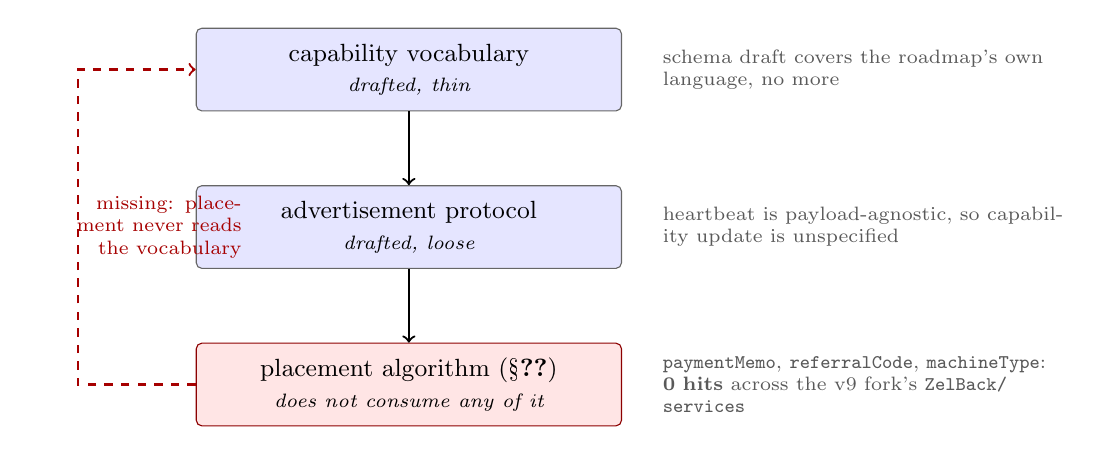
\begin{tikzpicture}[font=\small,
  box/.style={draw=black!60, rounded corners=2pt, minimum width=5.4cm, minimum height=1.05cm,
              align=center, inner sep=4pt},
  thin/.style ={box, fill=blue!10},
  loose/.style={box, fill=blue!10},
  none/.style ={box, fill=red!10, draw=red!55!black},
  note/.style ={font=\scriptsize, text=black!65, align=left, text width=5.1cm},
]
\node[thin]  (a) at (0,2.6) {capability vocabulary\\{\scriptsize\itshape drafted, thin}};
\node[loose] (b) at (0,0.6) {advertisement protocol\\{\scriptsize\itshape drafted, loose}};
\node[none]  (c) at (0,-1.4) {placement algorithm (\S\ref{sec:fluxos-placement})\\{\scriptsize\itshape does not consume any of it}};

\draw[->, thick] (a) -- (b);
\draw[->, thick] (b) -- (c);

% the missing feedback edge
%% Routed left: on the right it crossed the three grey annotation notes.
\draw[->, dashed, red!65!black, thick]
  (c.west) -- ++(-1.5,0) |- (a.west);
\node[font=\scriptsize, text width=2.6cm, align=right, text=red!65!black, anchor=east]
  at (-2.0,0.6) {missing: placement never reads the vocabulary};

\node[note, anchor=west] at (3.1,2.6)
  {schema draft covers the roadmap's own language, no more};
\node[note, anchor=west] at (3.1,0.6)
  {heartbeat is payload-agnostic, so capability update is unspecified};
\node[note, anchor=west] at (3.1,-1.4)
  {\texttt{paymentMemo}, \texttt{referralCode}, \texttt{machineType}: \textbf{0 hits} across the v9 fork's \texttt{Zel\allowbreak{}Back/\allowbreak{}services}};
\end{tikzpicture}

\caption{The three components a capability-typed provider runtime requires, and which of them exist
today.}
\end{figure}

\subsection{The datacenter tier and the field that names it}

The roadmap states its position on uniform capacity plainly, under the heading ``What we are not
doing'': ``\,`VPS on every node' in this cycle'' is rejected because ``home connections cannot serve
it reliably. The datacenter tier is what we can do properly now''
\srcroadmap{flux-roadmap-public.md:208}. That sentence has an architectural consequence the roadmap
does not spell out: a fleet that includes both home-connection Cumulus nodes and purpose-built
datacenter capacity is explicitly heterogeneous, and a specification that wants to route a workload
to one class and not the other has to say so. That is what \texttt{machineType} is for — a field on
the tenant side of the v9 schema that names \texttt{standard}, \texttt{gpu}, or \texttt{vps} as the
class of machine a deployment requires (\inprogress, \srccode{flux-spec/\allowbreak{}schema/\allowbreak{}v9.json}{79-82}).

The field is declared and unconsumed. As established above and in Section~10, \texttt{machineType}
has zero consumer code anywhere in \FluxOS, in either the organisation repository or its more mature
external fork. The VPS tier the roadmap schedules for H1~2027 is stated to depend on this exact flag
\srcroadmap{flux-roadmap-public.md:124-125}, and is itself gated behind the Q4~2026 operator-protection
work \srcroadmap{flux-roadmap-public.md:125}. So the tier has a name in the schema and nothing behind
it: no scheduling logic reads \texttt{machineType}, no node advertises which value it satisfies, and
no enforcement height is yet configured in \FluxOS{} for the specification version that carries the field, although one is now decided
(Section~10). Section~\ref{sec:feasibility} should carry this forward as one of the concrete, enumerable gaps between
the roadmap's dependency chain and what the code implements, rather than as a vague ``not yet
finished.''

\subsection{What convergence costs}

A single provider runtime is not free to build and would not be free to operate. The case for it is
real: one registration schema, one heartbeat mechanism, and one placement algorithm mean one code
path to secure and one place to add a new capability, instead of maintaining parity between \FluxOS's
gossip-based spawn loop and \FluxEdge's Kubernetes reconciler independently. A tenant who can express
\texttt{machine\allowbreak{}Type:\allowbreak{}~gpu} once and have it satisfied by whichever runtime currently holds the right
hardware gains something no product-level merge can deliver on its own — portability across a
heterogeneous fleet instead of a choice between two separately-billed products. The roadmap's ``payment
is the account, and per-second GPU without an account'' framing depends on exactly this: it is stated
to work ``with \FluxEdge folded into the platform'' \srcroadmap{flux-roadmap-public.md:79}, i.e. it
assumes the runtime-level unification this section has just shown is not yet designed.

The cost is that a single interface is shaped by its weakest supported node class. If the capability
vocabulary and placement algorithm are built to serve both a home-connection Cumulus node and a
datacenter-tier machine through one schema, either the interface degrades toward what the weaker class
can honestly promise, or the schema grows enough branching (as \texttt{machineType} already begins to
do) that ``one runtime'' becomes, in practice, several code paths gated by a flag — which is close to
where \FluxOS and \FluxEdge already are, just inside one repository instead of two. A home-connection
node and a datacenter node do not share a failure model: the roadmap's own reasoning for rejecting
``VPS on every node'' is precisely that home connectivity cannot be relied on for a workload class that
assumes always-on reachability \srcroadmap{flux-roadmap-public.md:208}. Any placement algorithm that
consumes capability flags has to encode that asymmetry correctly, or a tenant who requested
\texttt{vps} could in principle land on hardware whose network characteristics were never meant to
carry it — precisely the failure the tier distinction exists to prevent, and precisely the risk of
declaring a capability vocabulary before the placement algorithm that must honour it has been
designed.

\subsection{Vertical integration, argued both ways}

Flux controls the chain (\fluxd), the orchestration daemon (\FluxOS), and the attested host
(\ArcaneOS). One party controlling all three makes a guarantee reachable that no single-layer actor
could build alone: call it attested placement — a tenant's payment names a specific workload, \FluxOS
records which node placed it, and \ArcaneOS attests that the node booted a known-good image, with all
three artifacts meeting inside interfaces one party authors end to end.

No shipped mechanism assembles that chain today, and each leg is weaker than the phrase suggests.
The first leg does not yet exist: today a payment settles to a fixed transparent sink address and does
not reach the machine running the workload at all — the roadmap states this directly, ``today when
someone pays to run an application, that payment does not reach the machine running it''
\srcroadmap{flux-roadmap-public.md:111-112} — and binding a payment to a specific workload is exactly
what the PNR~v2 \texttt{paymentMemo} field is for (\planned; Section~7). The second leg is real but
off-chain: \FluxOS's placement decision is recorded in gossiped, signed messages, not on the chain
itself. The third leg exists but is weaker than ``attests the host'' implies: \ArcaneOS's attestation
service already defines a purpose-scoped signing key for exactly this use — a \texttt{purpose=app}
key sits alongside the existing, unconsumed \texttt{purpose=\allowbreak{}mesh} key
(\shipped, \srccode{fluxsas/\allowbreak{}src/\allowbreak{}api\_server.h}{411-481}) — but the signing material for every purpose
is derived by HKDF from salt and domain values compiled identically into every binary, not from
anything TPM- or machine-specific, so the attestation demonstrates that the signer holds a value
shipped in every copy of the software, not that a particular machine booted a particular image; there
is also no tenant-facing verification path today, since every attestation route requires an internal
mTLS client certificate bound to loopback. So ``attests the host'' is, at present, a Flux-operated
assurance a tenant cannot independently check, not a hardware-rooted one. The three names — the
payment-memo field, the placement gossip message, the attestation purpose token — are each Flux's own
schema decision; only a single controlling party is positioned to make them interoperate at all, which
is the sense in which the guarantee is uniquely reachable through vertical integration. Whether it is
actually reachable depends on work none of which has shipped: \vision, \srcinferred.

The same integration that makes this reachable has already foreclosed something else. The PoN block
header carries a fixed chainwork contribution per block regardless of difficulty
(\srccode{fluxd/\allowbreak{}src/\allowbreak{}pow.cpp}{284-290}), and a 2-of-4 emergency key set can produce a valid block
outside normal consensus rules. A header format chosen to make PoN's collateral-and-eligibility
sortition work is the same header format a light client on another chain would need to verify Flux
independently — and it cannot: without a commitment to the node set, without cumulative work to
compare forks by, and with an emergency path that can override normal validity, no light-client rule
derived from this header is sound. The most trust-minimising bridge architecture available to other
chains is closed to Flux until the header changes \srcintent{plan/mech-bridge.md, \S22}. That is the
same asymmetry as the attested-placement argument, run in the other direction: a design decision made
because one party controlled the whole stack, for one purpose, closed an option for a different
purpose that a less integrated system might have kept open. Integration is not, on this evidence, a
virtue or a defect on net; it is a set of coupled decisions with gains on one axis and closed doors on
another, and this section states both rather than choosing one.

\subsection{What would make convergence checkable}

Three things would turn this from an architectural claim into a testable one. First, a published
capability vocabulary — not the three-flag \texttt{capabilities} object and the three-value
\texttt{machineType} enum as they stand, but a vocabulary that actually covers GPU class, network
grade and storage durability, published somewhere a second implementation could target without
vendoring a private repository. Second, a placement algorithm — whether a revision of Section~9's
spawn loop or a successor — that reads that vocabulary when choosing a node, rather than the current
mechanism, which ignores every field convergence would depend on. Third, an enforcement height in the shipped configuration: v9 has
none today, though Section~10 records the one the team has settled on, and neither the provider-runtime contract nor the application schema that
carries \texttt{machineType} becomes binding on the network until one is set. Until all three exist,
``one platform'' describes an intent the roadmap has stated clearly and a runtime the code has not yet
built.

%% Drain this section's float queue before the next begins.
\FloatBarrier
